%! Author = adnansiddiquei
%! Date = 07/12/2023

% Preamble
\documentclass[a4paper,11pt]{article}
\pdfoutput=1

% Packages
\usepackage{jcappub}
\usepackage[T1]{fontenc}
\usepackage{listings}
\usepackage{roboto}
\usepackage{subcaption}

\newcommand{\inlinecode}[1]{\lstinline{#1}}
\lstset{basicstyle=\fontfamily{pcr}\selectfont}


\title{\boldmath An implementation of a python sudoku solver package and a complete review of the software development
process involved.}


% %simple case: 2 authors, same institution
 \author{Adnan Siddiquei}
 \affiliation{University of Cambridge}

% e-mail addresses: one for each author, in the same order as the authors
\emailAdd{as3438@cam.ac.uk}




%\abstract{Abstract...}



\begin{document}
\maketitle
\flushbottom

\section{Introduction}\label{sec:intro}

%! Author = adnansiddiquei
%! Date = 07/12/2023

\section{Solution Design}\label{sec:solution-design}
    \subsection{Prototyping}\label{subsec:prototyping}
    Prior to writing any code, we prototyped the solution.
    Prototyping prior to coding allowed us to
    \begin{itemize}
        \item identify possible bugs and complexity earlier on in the development process, such that we could consider them
        prior to coding, rather than discover them after the fact;
        \item identify non-trivial and edge cases that might need to be considered while writing code and unit tests;
        \item identify API interfaces of the package, allowing us to write the unit tests beforehand (more on this when
        we talk about test driven development in Section\eqref{subsec:test-driven-development}).
        \item explore different implementations of the backtracking algorithm;
        \item identify python packages and resources that we may need to use in the implementation, and make decisions on which
        might be the most appropriate;
    \end{itemize}
    The implementation of the sudoku solver consisted of two main components: parsing the user input (and handling
    associated errors), and the backtracking algorithm itself.
    The prototyping flowcharts of these two components is shown in Fig.\eqref{fig:input-prototype} and Fig.\eqref{fig:backtracking-prototype}.
    Additionally, we wrote some \textit{pseudo-python-code} as shown in Fig.\eqref{fig:pseudocode}, allowing us to define
    the interfaces of the functions and classes that we would write - which is required to write any unit tests before prior
    to coding.
    The tests derived from this solution design are discussed more in Section\eqref{sec:validation-unit-tests-and-ci-set-up}.
    Further iterations on these initial prototypes are discussed more in Section\eqref{sec:development-experimentation-and-profiling}
    where we discuss how experimentation and profiling changed the end implementation in efforts to optimise the code.

    \subsection{API Interface}\label{subsec:api-interface}
    An important decision to make early on is how the code will be structured into modules and what the external
    API interface will look like, as shown in Fig.\eqref{fig:pseudocode}.
    We decided to model the \inlinecode{sudokusolver} package after well known \inlinecode{scikit-learn} \cite{scikit-repo}
    package because \inlinecode{scikit-learn}'s structure is extremely well thought out and simple to use.
    Each solver would be segmented into a class which can be instantiated with the hyperparameters
    of the solver (in this case, is there \inlinecode{multiple_solutions}), and then a \inlinecode{solve} method which
    takes in the data (the \inlinecode{unsolved_board}) and returns the class instance with the solved board as an attribute.
    This seemed like a fitting way to model the package as our solvers are akin to \inlinecode{scikit-learn}'s estimators,
    and the \inlinecode{solve} method is akin to \inlinecode{scikit-learn}'s \inlinecode{fit} method.
    To extend the package we simply need to add more solvers classes, and to extend a solver we simply need
    to add more hyperparameters to the class and modify the \inlinecode{solve} method to take these hyperparameters into
    account.

    \subsection{Key Conclusions}\label{subsec:key-conclusions}
    We decided to only implement the \inlinecode{BacktrackingSolver} with no \inlinecode{multiple_solutions} functionality
    in the initial \inlinecode{v1.0.0} implementation of the package,
    The implementation of \inlinecode{multiple_solutions} was not thought through in the prototyping stage but given that
    we now understood how to syntactically and structurally extend the package and the solvers within, it would be trivial
    to add this functionality in a future version of the package, which demonstrates the importance of blueprinting out
    the API interface.

    Another key decision which was implicit and not thoroughly discussed was to utilise \inlinecode{numpy} arrays to
    represent the sudoku board, this is because \inlinecode{numpy} is well known to be the most performant array manipulation
    package in python.
    Alternatives include using \inlinecode{pandas} or python's in-built \inlinecode{list} object, however, \inlinecode{numpy}
    is generally known to be more performant than both of these and \inlinecode{numpy} also includes numerous built-in functions
    that will be useful in the implementation of the backtracking algorithm.

    \begin{figure}[htb]
    \centering
    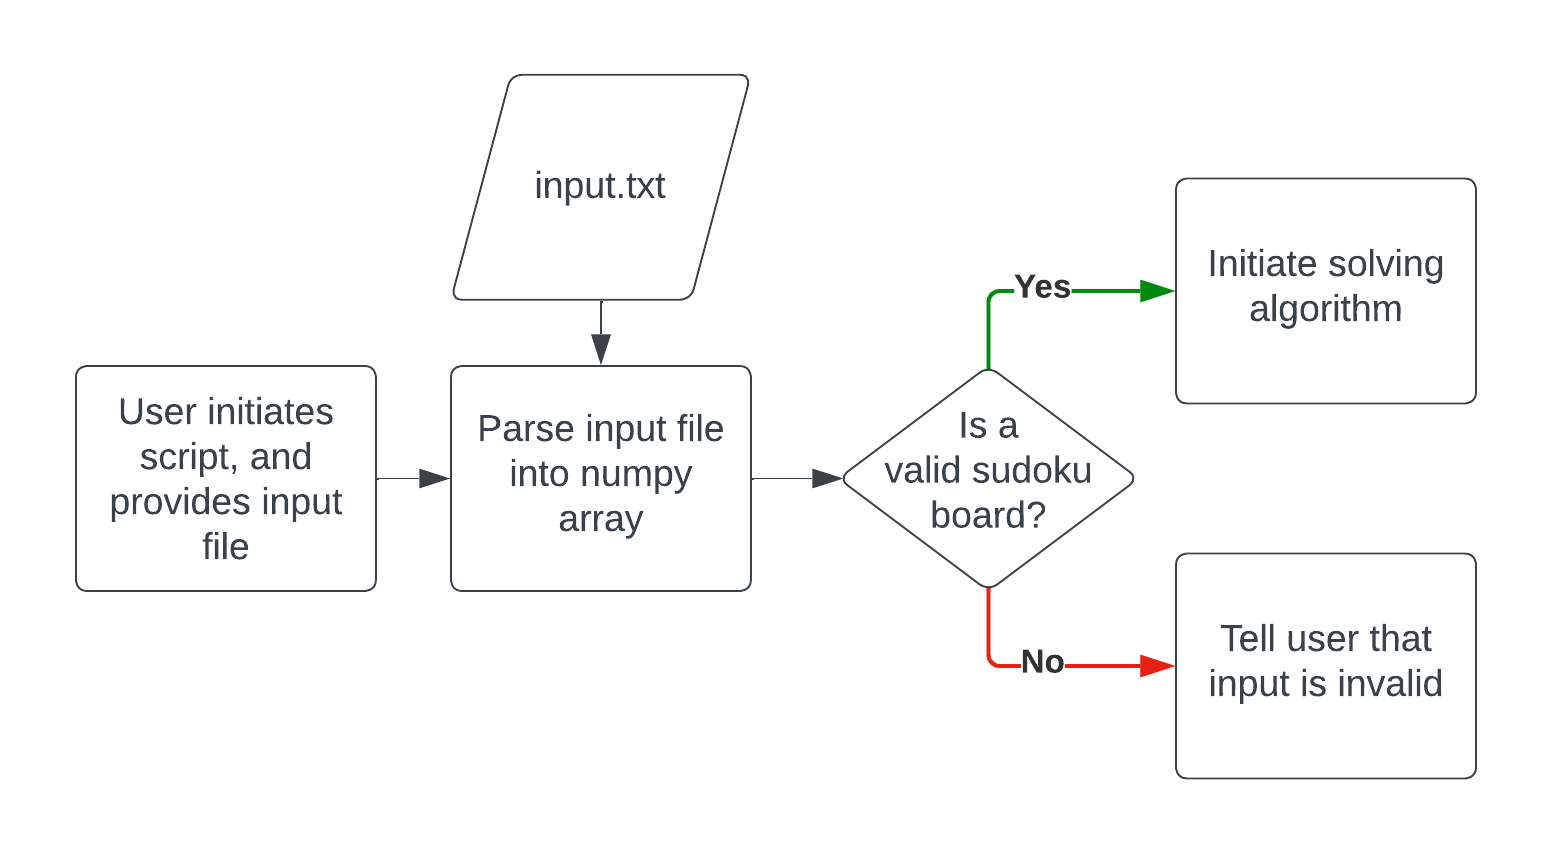
\includegraphics[width=0.9\textwidth]{./figures/parse-input-prototype}
    \caption{A flowchart for part 1 of solving a sudoku puzzle: parsing the user input.}
    \label{fig:input-prototype}
    \end{figure}

    \begin{figure}[htb]
    \centering
    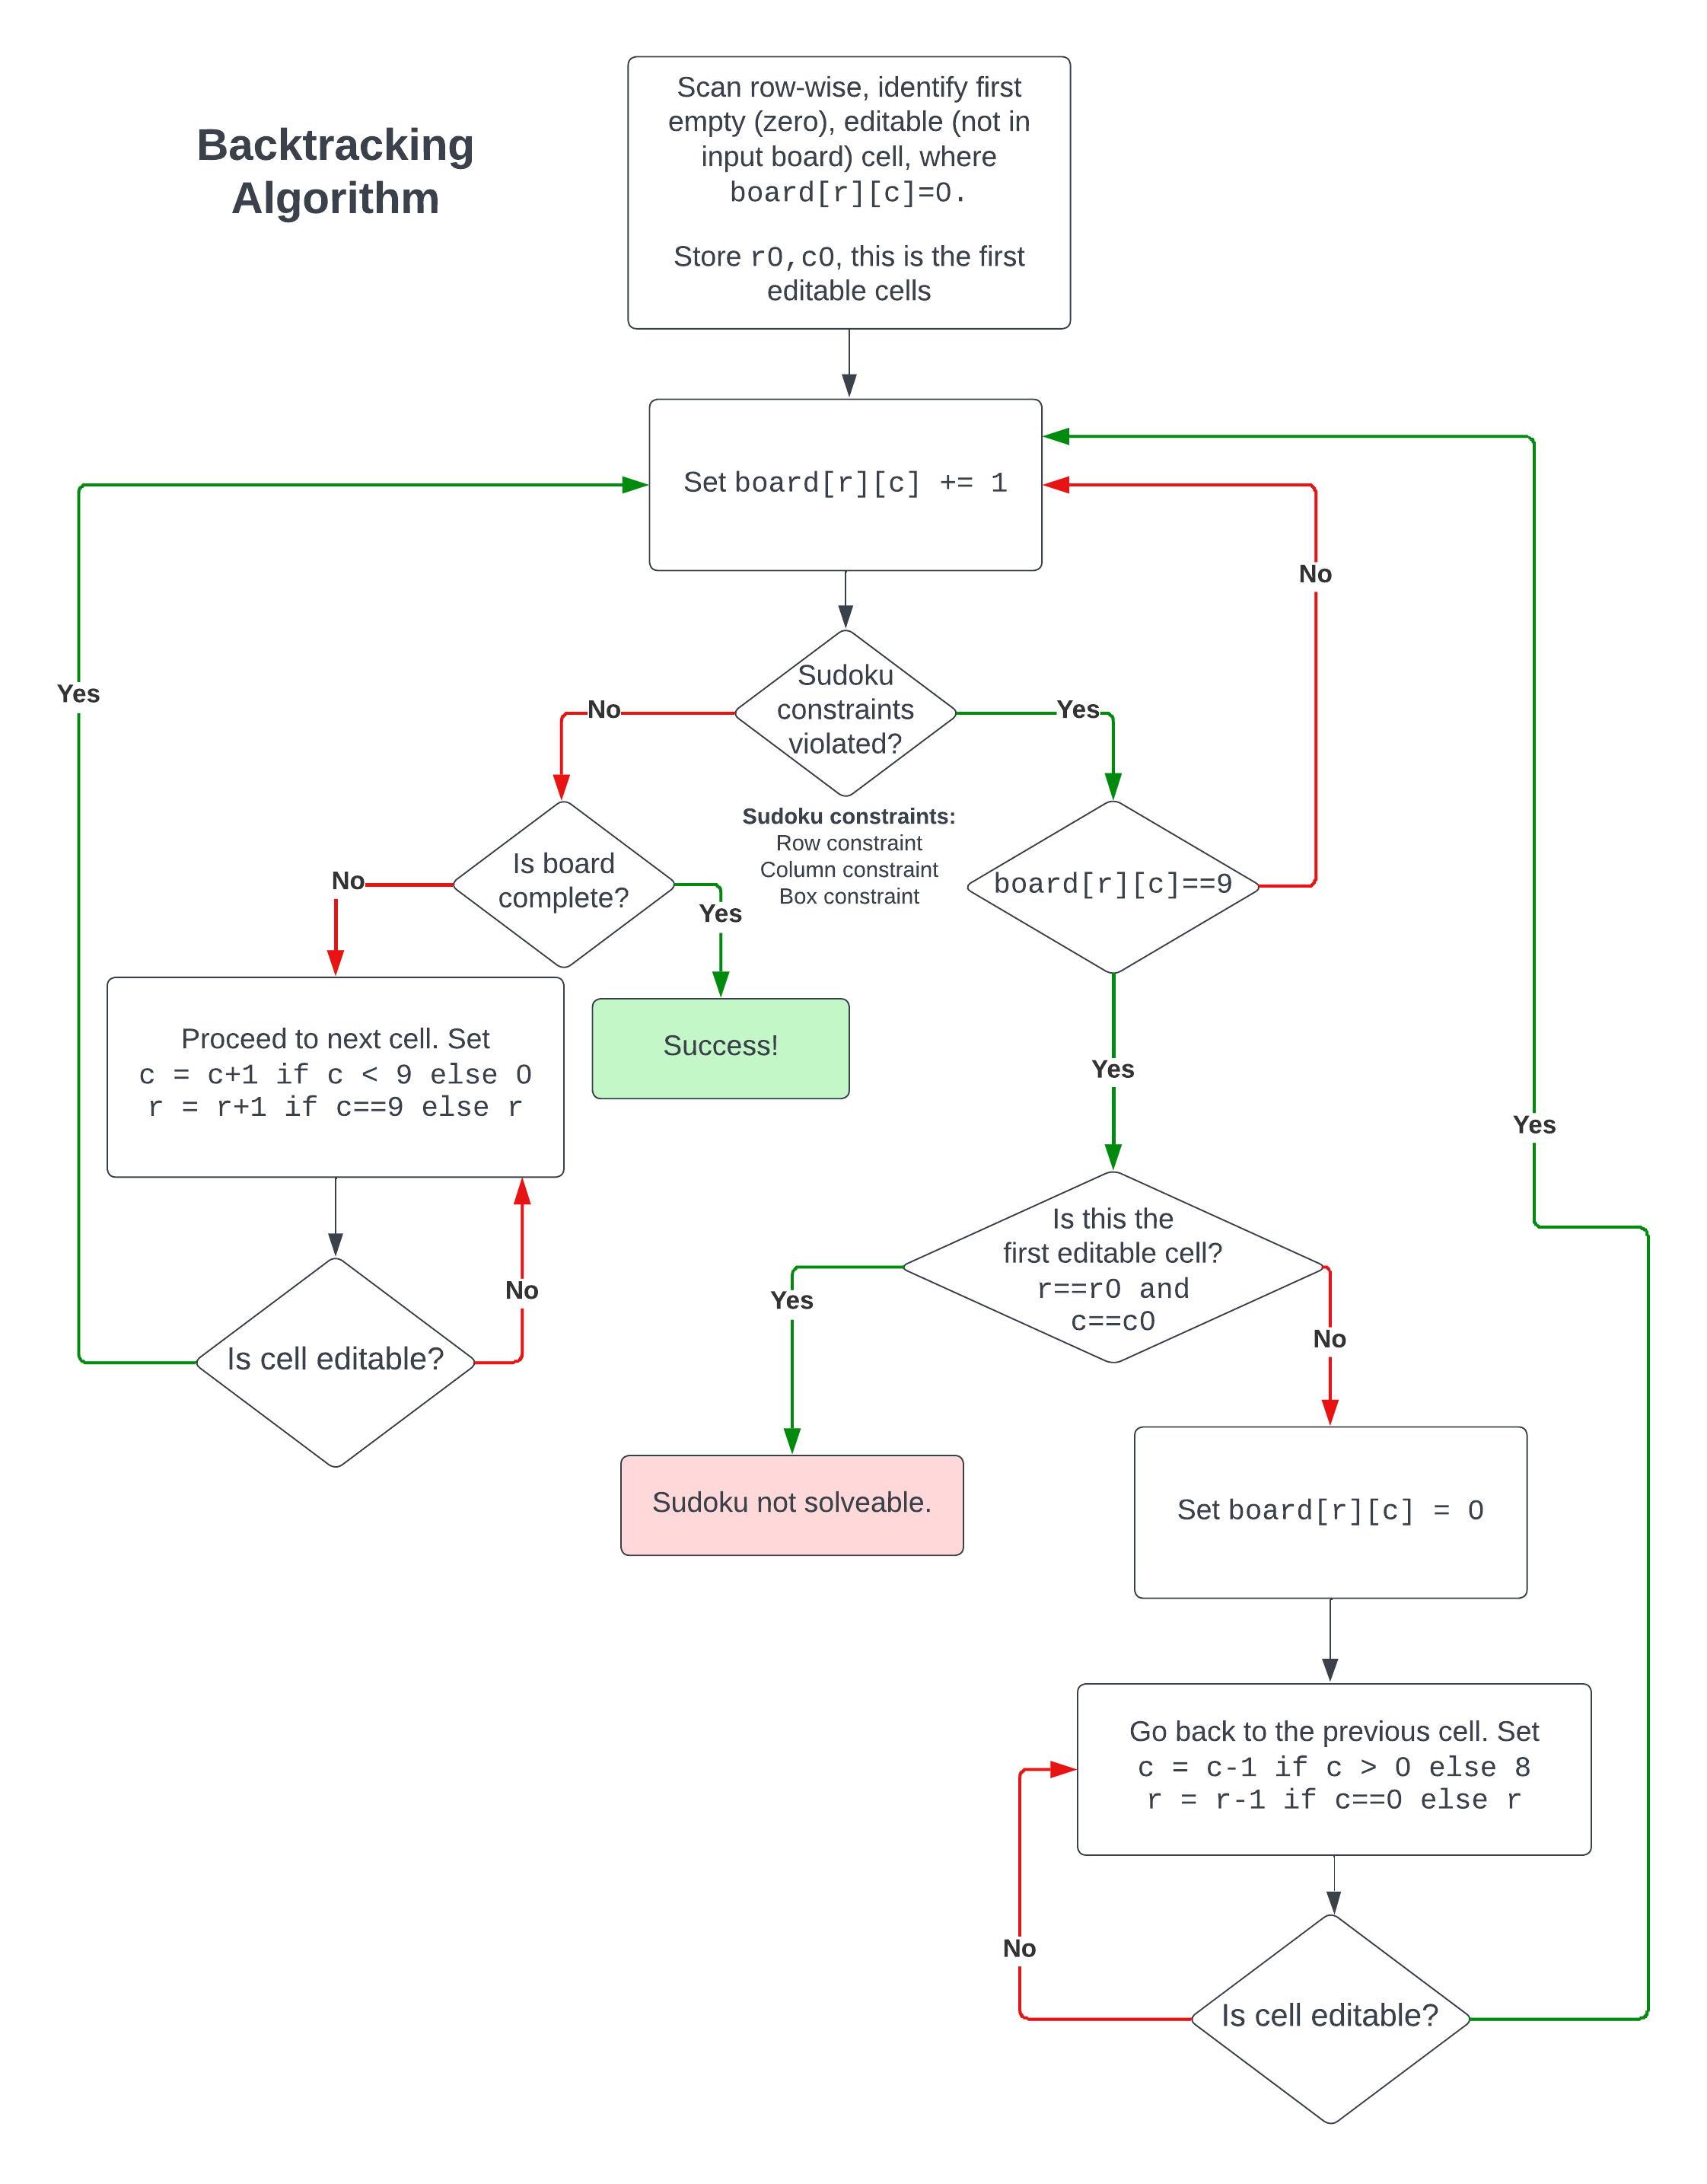
\includegraphics[width=0.9\textwidth]{./figures/backtracking-prototype}
    \caption{A flowchart for part 2 of solving a sudoku puzzle: the backtracking algorithm.}
    \label{fig:backtracking-prototype}
    \end{figure}

    \begin{figure}[htb]
    \centering
    \begin{lstlisting}[language=Python,label={lst:lstlisting}]
        class BacktrackingSolver
            def __init__(self, multiple_solutions: bool = False):
                self.board  # will store solved board
                self.is_solved  # will store whether board is solved
                self.is_solvable  # will store whether board is solvable
                self.is_valid  # will store whether board is valid
            def solve(self, unsolved_board: numpy.NDArray):

        def parse_input_file(input_file_path: str) -> numpy.NDArray

        def save_board_to_txt(
            board: numpy.NDArray,
            output_file_path: str
        ) -> None

        # entry point for script, argv = sys.argv
        def handler(argv) -> None:
    \end{lstlisting}
    \caption{\textit{pseudo-python-code} representation of the interfaces of the functions and classes within our
    \inlinecode{sudokusolver} package.}
    \label{fig:pseudocode}
    \end{figure}


%! Author = adnansiddiquei
%! Date = 07/12/2023

\section{Development, Experimentation and Profiling}\label{sec:development-experimentation-and-profiling}
Here we discuss several components of the development process, and reason why we chose to do things in certain ways

\subsection{Linting and Formatting - \inlinecode{ruff}}\label{subsec:linting-and-formatting}
    Linting and formatting is useful, especially in shared projects, as it allows for a consistent style across the codebase.
    There are a plethora of python linting and formatting tools available and for this project, we chose to use \inlinecode{ruff}.
    There were two primary reasons for this choice: speed and simplicity.
    \inlinecode{ruff} is faster than most other linting tools including \inlinecode{flake8}.
    In a test done by the developers of \inlinecode{ruff}, it managed to lint the CPython codebase 42x faster than
    \inlinecode{flake8} \cite{ruff-repo}.
    Whilst speed of linting is not a primary concern for this project, it doesn't hurt to pick the faster option.

    Additionally, \inlinecode{ruff} provides formatting functionality and as such it can also replace tools such as
    \inlinecode{black}.
    This makes the implementation of linting and formatting simpler, as we only need to use one tool.
    \inlinecode{ruff}'s configuration capabilities allow it to lint and format to any standard we want to, and as such,
    it was configured to mimic \inlinecode{black} and \inlinecode{flake8}'s default config in accordance with PEP8.

    \subsection{Git and Gitlab Workflows}\label{subsec:git-and-gitlab-pipeline}
    It is generally good practise to write detailed commit messages and merge requests, and traditionally in larger
    software projects, project management tools such as JIRA are used to track issues and tasks, and merge requests
    are linked to these issues.
    In the world of open source, and small projects like this, GitLab's issue tracker works as a perfect tool for this.
    Therefore, we utilised the issue tracker to create issues for tasks that needed to be done, and then linked merge requests
    to these issues.
    In this way, we could maintain detailed documentation in the issue tracker of what was done, and why it was done,
    in a slightly more structured way than just using commit messages.
    Therefore, a new branch was created for every issue, and once the branch implemented or resolved the features in the
    issue, a merge request was created, linked to the issue, merged into main, and the issue was closed.
    As such, anyone with access to the repo can see the git commit history through the GitLab UI and any references to issue
    numbers in commits can be clicked to link the user to the underlying issue which describes what was implemented and why.

    Furthermore, a nice feature of many project management tools and IDE's is the ability to group branches into folders
    based on the branch name.
    Git allows forward slashes '/' in branch names such that branches can be structured into folders by the IDE, as such
    a naming convention was adopted for branches.
    Branches were named like the following: \inlinecode{feat/issue-1} or \inlinecode{tests/issue-4} where the 3 main
    'folders' used were \inlinecode{feat} for feature, \inlinecode{tests} and \inlinecode{bug}, followed by
    the issue number it implemented.
    In practise, the \inlinecode{bug} folder was not used as bugs as no bugs were discovered.
    Occasionally a \inlinecode{report} branch was created when only the report needed to be updated, these were not linked
    to any issues.

    Overall, these Git and GitLab workflows allowed for a structured development process, and a detailed history of
    what was done and why it was done, which is useful for future reference.

    \subsection{Test Driven Development}\label{subsec:test-driven-development}
    Where possible, we strived to do test driven development by writing tests first.
    This was made possible due to the careful prototyping and API design discussed in Section\eqref{sec:solution-design}.
    The reason we decided to write tests first came from three primary reasons:
    \begin{itemize}
        \item it streamlined code writing, as we were already aware of what the code needed to do, and what the edge cases
        were.
        \item it defined clearly what the end product would be;
        \item it reduced debugging time.
        We could more quickly figure out what was going wrong if a bug arose;
    \end{itemize}
    The final tests that were written are discussed more in Section\eqref{sec:validation-unit-tests-and-ci-set-up}.

    \subsection{Profiling and Optimisation [TODO]}\label{subsec:profiling-and-optimisation}
    Where did i test different packages for speed? Why did I choose numpy?
    Show how I profiled my code to identify where the bottleneck was.
    How did I work around this? Cython?

    \subsection{Coding Best Practises [TODO]}\label{subsec:coding-best-practises}
    Modularisation.
    typing.
    Exceptions. Error handling, try except. Never catch all exceptions.



\section{Validation, Unit Tests and CI set up [TODO]}\label{sec:validation-unit-tests-and-ci-set-up}
Talk through why my unit tests are sufficient.
How did I put this into the CI? With pre-commit.yaml

%! Author = adnansiddiquei
%! Date = 08/12/2023

\section{Documentation, Packaging and Usability}\label{sec:documentation-packaging-and-usability}
    \subsection{Documentation - \inlinecode{sphinx} and NumPy Style Docstrings}\label{subsec:documentation-sphinx}
    Documentation is an important part of any software project, without it, the user would have no idea how to utilise
    third-party packages.
    Documentation comes in two forms: inline documentation (docstrings and comments) and usage documentation (user guides
    and API references).
    The former is written whilst developing the code, and the latter is generated from the former with documentation tools.

    The discussion of which documentation tool to use is quite an opinionated one, there is no strict "one is better than
    the other" in most cases.
    The two most popular ones in python are \inlinecode{sphinx} and \inlinecode{doxygen}.
    Whilst using either of these tools would have been sufficient, \inlinecode{sphinx} was chosen for this project
    primarily because of the vast universe of themes and extensions available for it.
    The reason for documentation is to help a user understand how to use the package, and as such, above all else
    the documentation output should be easy to read and navigate.
    \inlinecode{sphinx} has a number of themes available, and the one chosen for this project was \inlinecode{furo} which
    is used by \inlinecode{pip} \cite{pip-docs}\, \inlinecode{black} \cite{black-docs} and the python developer's guide
    \cite{python-devguide}.
    Whilst the setup for \inlinecode{sphinx} was a bit more hands on, it resulted in much more usable and aesthetic docs.

    Another motivator for using \inlinecode{sphinx} was the ability to use NumPy style docstrings.
    More so than the desire to use NumPy style docstrings, was the desire to not use Epytext style or reStructuredText style
    docstrings, which is what Doxygen requires.
    We found these styles to be much less readable than NumPy style docstrings, which was another motivator for using
    \inlinecode{sphinx}.
    Another popular alternative is Google style doctrings, NumPy style was chosen only by personal preference, \inlinecode{sphinx}
    can handle both.

    \subsection{Packaging - Conda and Docker [TODO]}\label{subsec:packaging-pypi}
    What benefits does conda have over pip? Why did I choose conda?
    Why Docker?


\section{Summary [TODO]}\label{sec:summary}


\begin{thebibliography}{99}

\bibitem{ruff-repo}
Astral,
\textit{\inlinecode{ruff} GitHub Repository}.
Available at: \url{https://github.com/astral-sh/ruff}
[Accessed: 7-Dec-2023].

\bibitem{scikit-repo}
scikit-learn,
\textit{\inlinecode{schikit-learn} GitHub Repository}.
Available at: \url{https://github.com/scikit-learn/scikit-learn}
[Accessed: 7-Dec-2023].

\bibitem{pip-docs}
The pip developers,
\textit{pip docs}.
Available at: \url{https://pip.pypa.io/en/stable/}
[Accessed: 8-Dec-2023].

\bibitem{black-docs}
Lukasz Langa and contributors to Black,
\textit{Black docs}.
Available at: \url{https://black.readthedocs.io/en/stable/}
[Accessed: 8-Dec-2023].

\bibitem{python-devguide}
Python Software Foundation,
\textit{Python Developer's Guide}.
Available at: \url{https://devguide.python.org/}
[Accessed: 8-Dec-2023].

\end{thebibliography}



\end{document}
